\documentclass[11pt]{article}
\usepackage[textwidth=18.0cm, textheight=23.0cm, top=2.0cm]{geometry}
\usepackage{pst-all}
\usepackage{amssymb}
\usepackage{tikz}
\usepackage{underscore}\begin{document}
\pagestyle{empty}


ClassName: \underline{\textbf{Class_05.2bp-15}}
\par
BinSize: \underline{\textbf{100 × 100}}
\par
ReduceSize: \underline{\textbf{100 × 100}}
\par
TypeNum: \underline{\textbf{40}}
\par
Num: \underline{\textbf{40}}
\par
OutS: \underline{\textbf{120000}}
\par
InS: \underline{\textbf{87773}}
\par
Rate: \underline{\textbf{0.731}}
\par
UB: \underline{\textbf{12}}
\par
LB0: \underline{\textbf{12}}
\par
LB: \underline{\textbf{12}}
\par
LBWithCut: \underline{\textbf{12}}
\par
NodeCut: \underline{\textbf{0}}
\par
ExtendedNodeCnt: \underline{\textbf{1}}
\par
GenNodeCnt: \underline{\textbf{1}}
\par
PrimalNode: \underline{\textbf{0}}
\par
ColumnCount: \underline{\textbf{12}}
\par
TotalCutCount: \underline{\textbf{0}}
\par
RootCutCount: \underline{\textbf{0}}
\par
LPSolverCnt: \underline{\textbf{1}}
\par
PricingSolverCnt: \underline{\textbf{0}}
\par
BranchAndBoundNum: \underline{\textbf{1}}
\par
isOpt: \underline{\textbf{true}}
\par
TimeOnInitSolution: \underline{\textbf{0.000 s}}
\par
TimeOnPrimal: \underline{\textbf{0.000 s}}
\par
TimeOnPricing: \underline{\textbf{0.000 s}}
\par
TimeOnRmp: \underline{\textbf{0.094 s}}
\par
TotalTime: \underline{\textbf{0.172 s}}
\par
\newpage


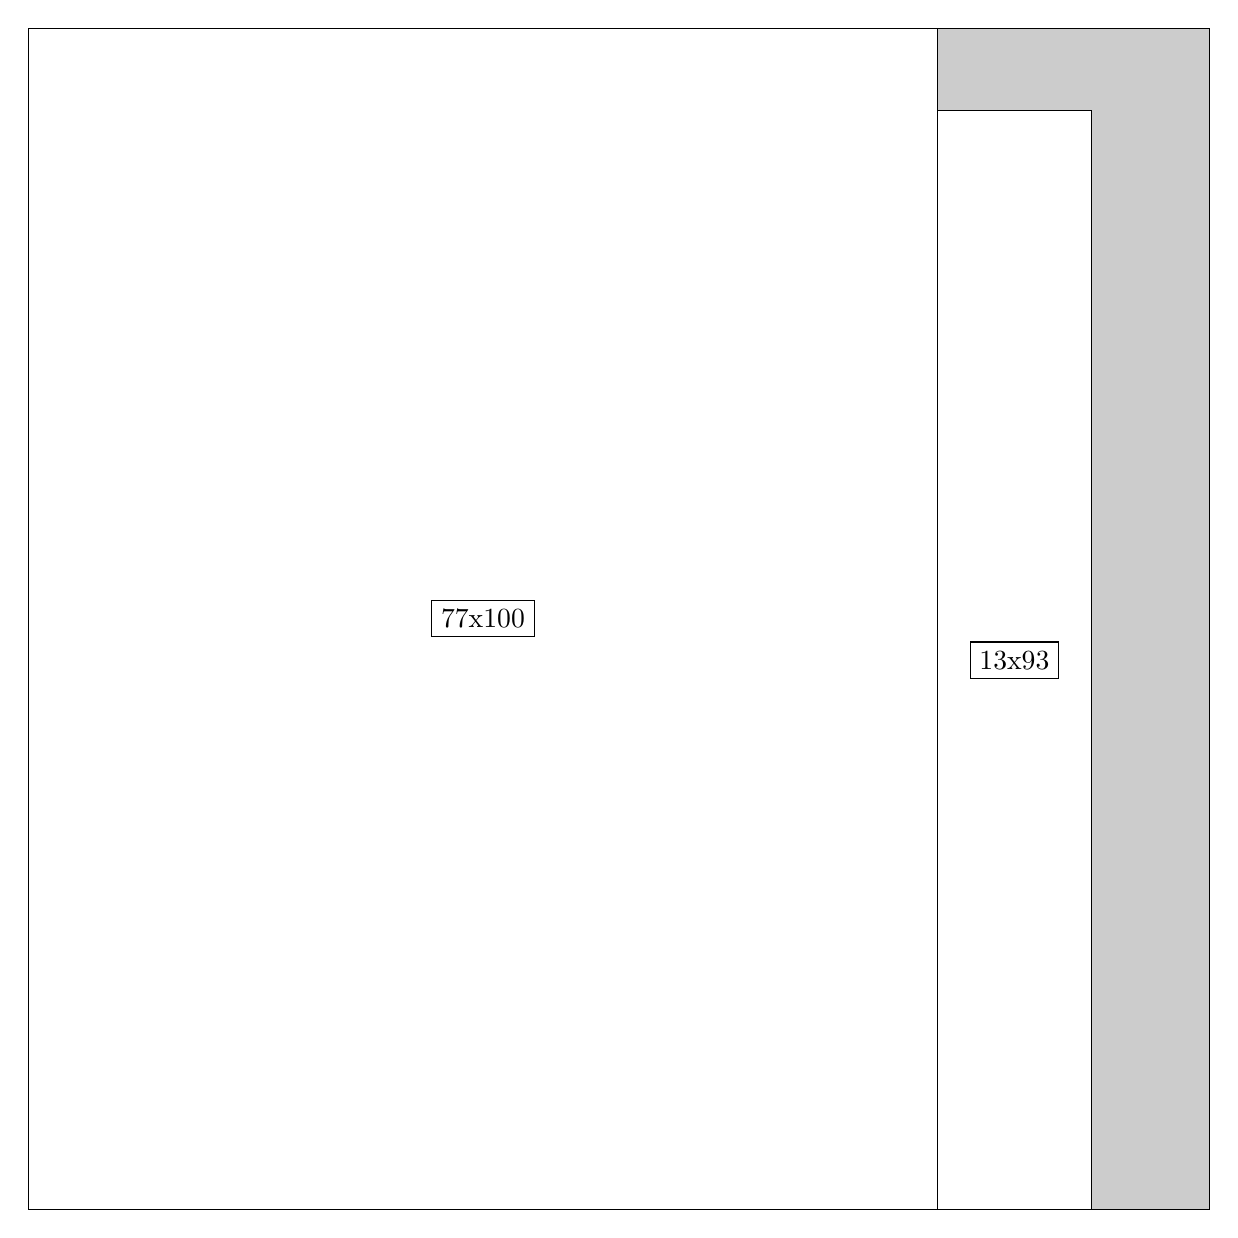
\begin{tikzpicture}[shorten >=1pt,scale=1.0,every node/.style={scale=1.0},->]
\tikzstyle{vertex}=[circle,fill=black!25,minimum size=14pt,inner sep=0pt]
\filldraw[fill=gray!40!white, draw=black] (0,0) rectangle (15.0,15.0);
\foreach \name/\x/\y/\w/\h in {77x100/0.0/0.0/11.549999999999999/15.0,13x93/11.549999999999999/0.0/1.95/13.95}
\filldraw[fill=white!40!white, draw=black] (\x,\y) rectangle node[draw] (\name) {\name} ++(\w,\h);
\end{tikzpicture}


w =77 , h =100 , x =0 , y =0 , v =7700
\par
w =13 , h =93 , x =77 , y =0 , v =1209
\par
\newpage


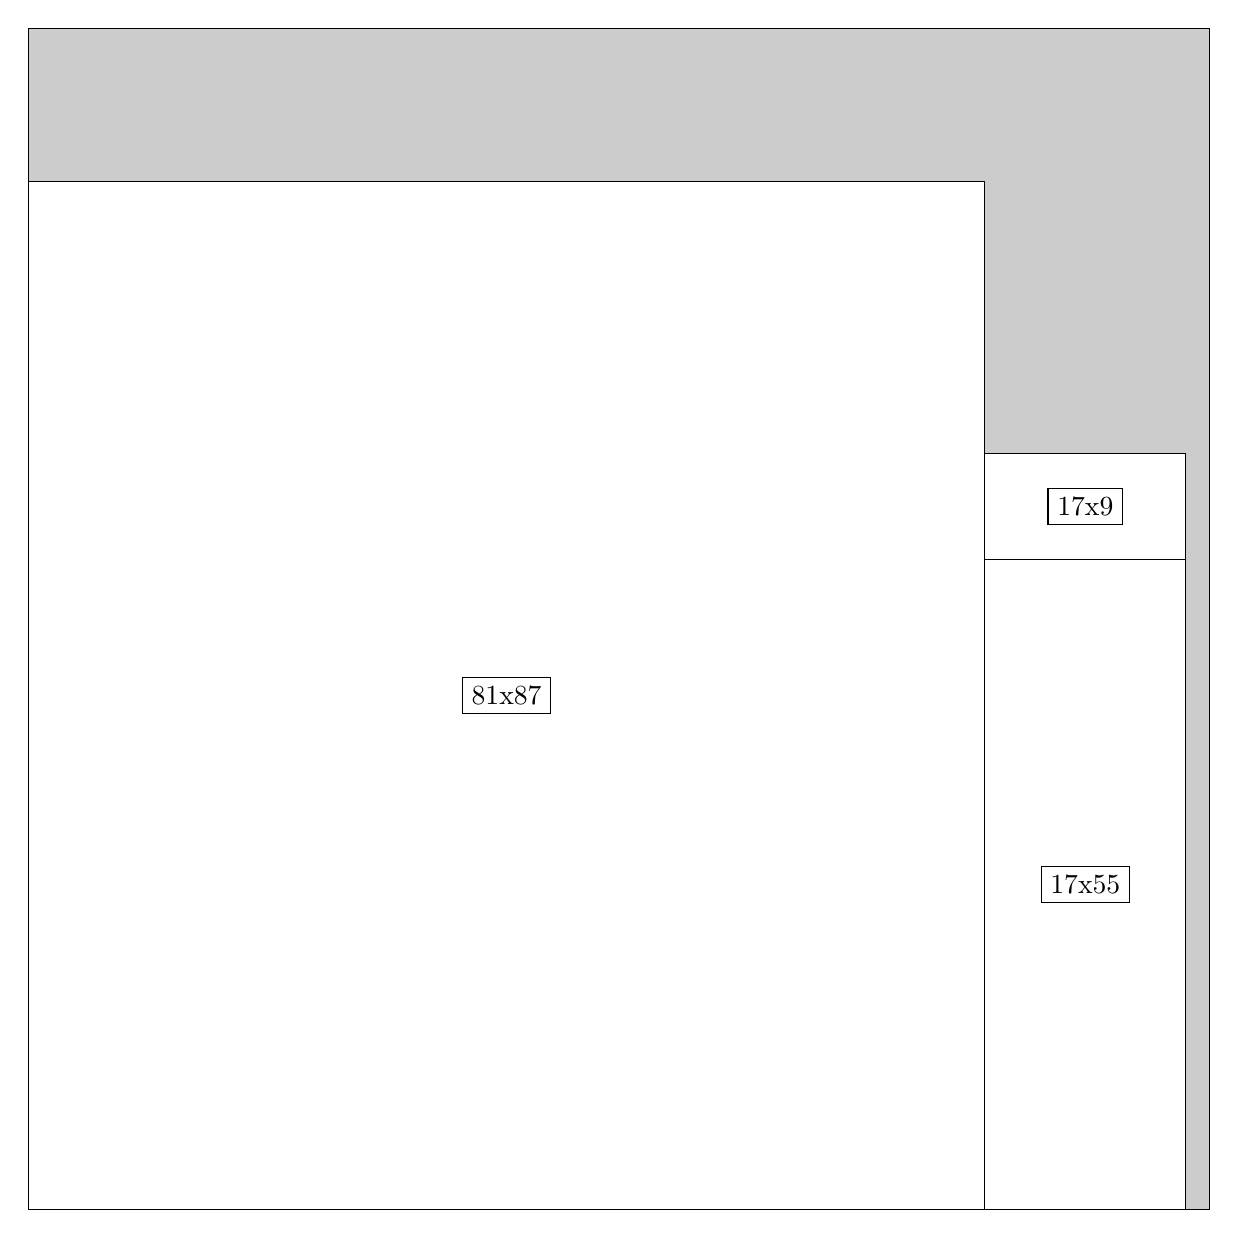
\begin{tikzpicture}[shorten >=1pt,scale=1.0,every node/.style={scale=1.0},->]
\tikzstyle{vertex}=[circle,fill=black!25,minimum size=14pt,inner sep=0pt]
\filldraw[fill=gray!40!white, draw=black] (0,0) rectangle (15.0,15.0);
\foreach \name/\x/\y/\w/\h in {81x87/0.0/0.0/12.15/13.049999999999999,17x55/12.15/0.0/2.55/8.25,17x9/12.15/8.25/2.55/1.3499999999999999}
\filldraw[fill=white!40!white, draw=black] (\x,\y) rectangle node[draw] (\name) {\name} ++(\w,\h);
\end{tikzpicture}


w =81 , h =87 , x =0 , y =0 , v =7047
\par
w =17 , h =55 , x =81 , y =0 , v =935
\par
w =17 , h =9 , x =81 , y =55 , v =153
\par
\newpage


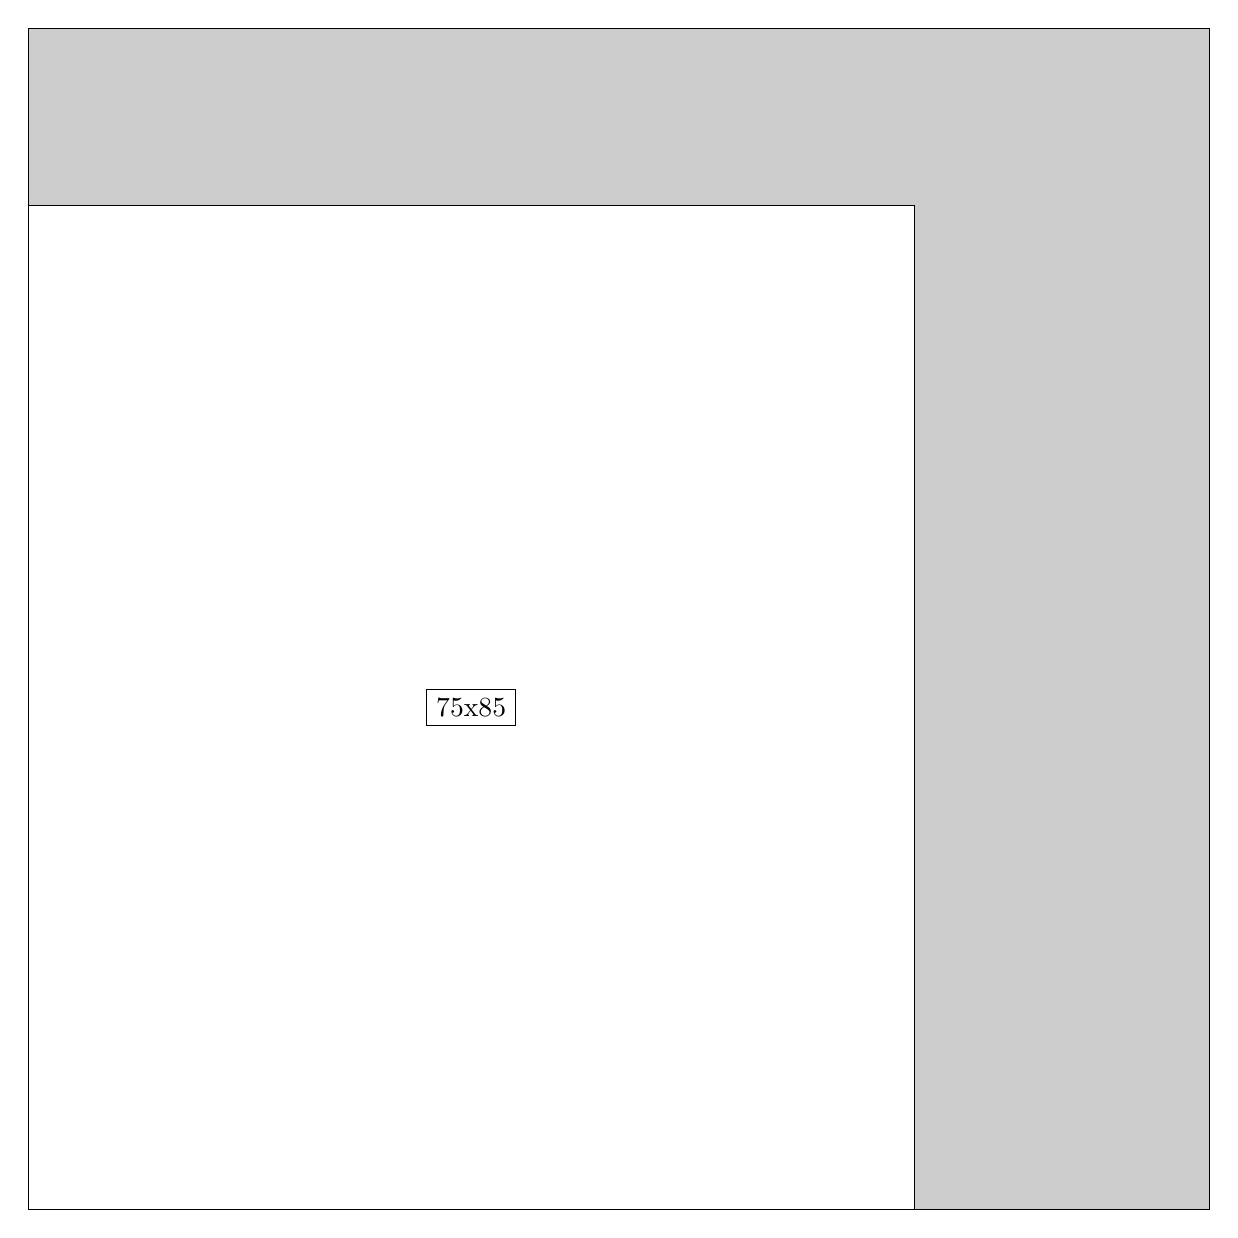
\begin{tikzpicture}[shorten >=1pt,scale=1.0,every node/.style={scale=1.0},->]
\tikzstyle{vertex}=[circle,fill=black!25,minimum size=14pt,inner sep=0pt]
\filldraw[fill=gray!40!white, draw=black] (0,0) rectangle (15.0,15.0);
\foreach \name/\x/\y/\w/\h in {75x85/0.0/0.0/11.25/12.75}
\filldraw[fill=white!40!white, draw=black] (\x,\y) rectangle node[draw] (\name) {\name} ++(\w,\h);
\end{tikzpicture}


w =75 , h =85 , x =0 , y =0 , v =6375
\par
\newpage


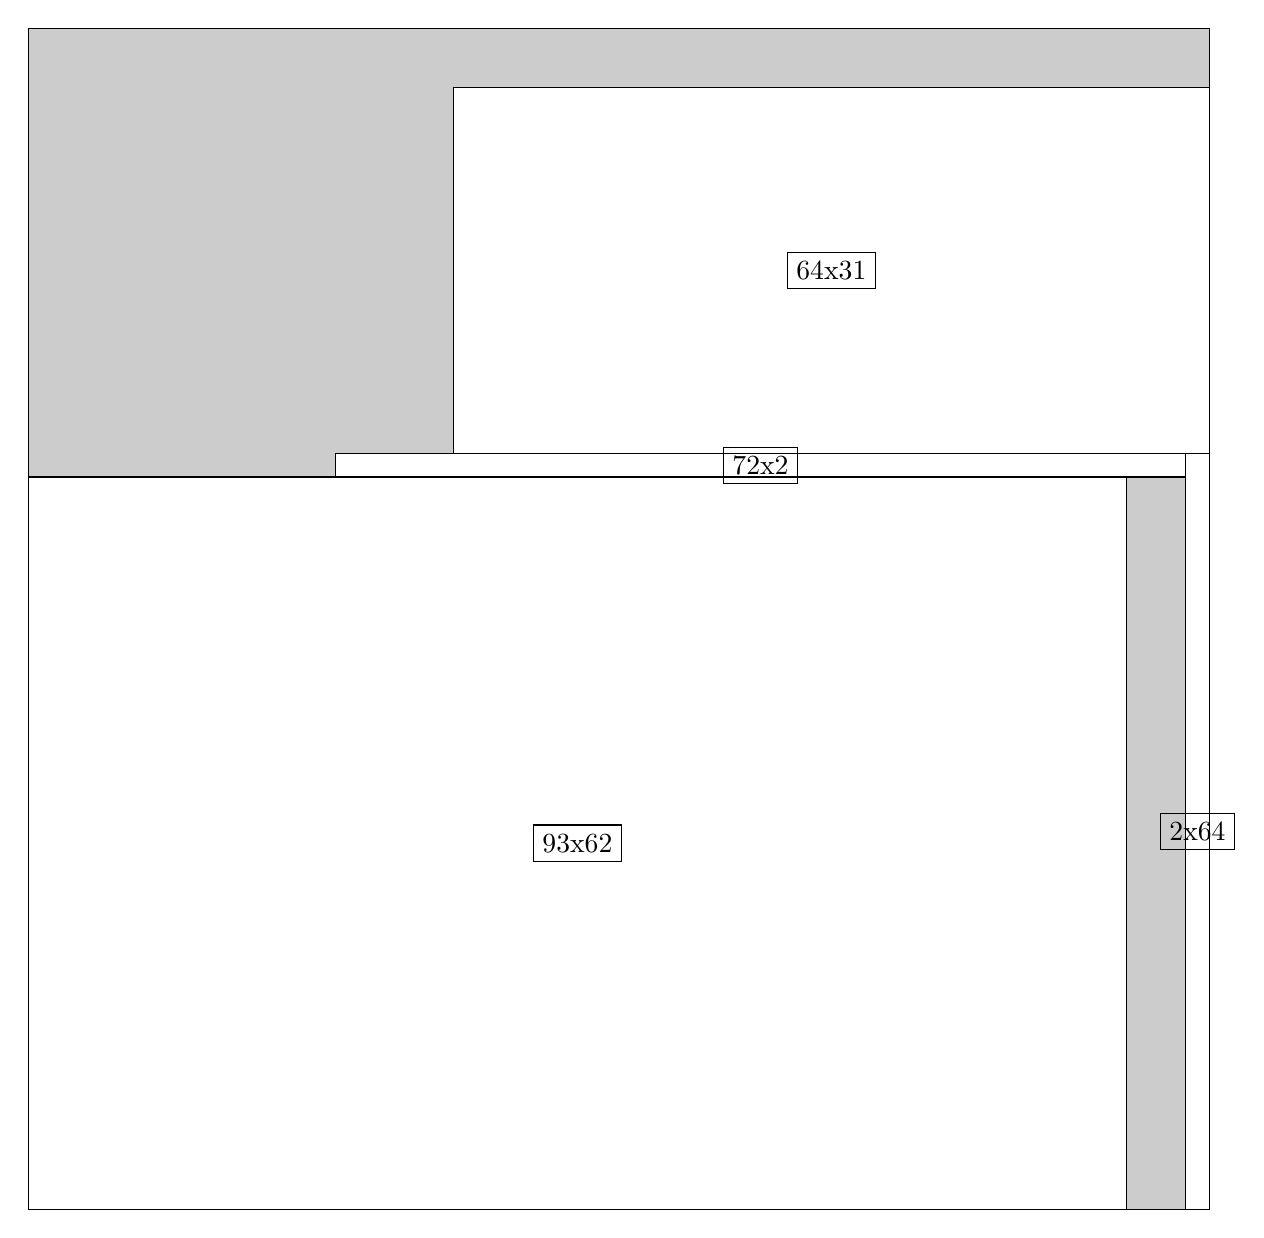
\begin{tikzpicture}[shorten >=1pt,scale=1.0,every node/.style={scale=1.0},->]
\tikzstyle{vertex}=[circle,fill=black!25,minimum size=14pt,inner sep=0pt]
\filldraw[fill=gray!40!white, draw=black] (0,0) rectangle (15.0,15.0);
\foreach \name/\x/\y/\w/\h in {93x62/0.0/0.0/13.95/9.299999999999999,64x31/5.3999999999999995/9.6/9.6/4.6499999999999995,72x2/3.9/9.299999999999999/10.799999999999999/0.3,2x64/14.7/0.0/0.3/9.6}
\filldraw[fill=white!40!white, draw=black] (\x,\y) rectangle node[draw] (\name) {\name} ++(\w,\h);
\end{tikzpicture}


w =93 , h =62 , x =0 , y =0 , v =5766
\par
w =64 , h =31 , x =36 , y =64 , v =1984
\par
w =72 , h =2 , x =26 , y =62 , v =144
\par
w =2 , h =64 , x =98 , y =0 , v =128
\par
\newpage


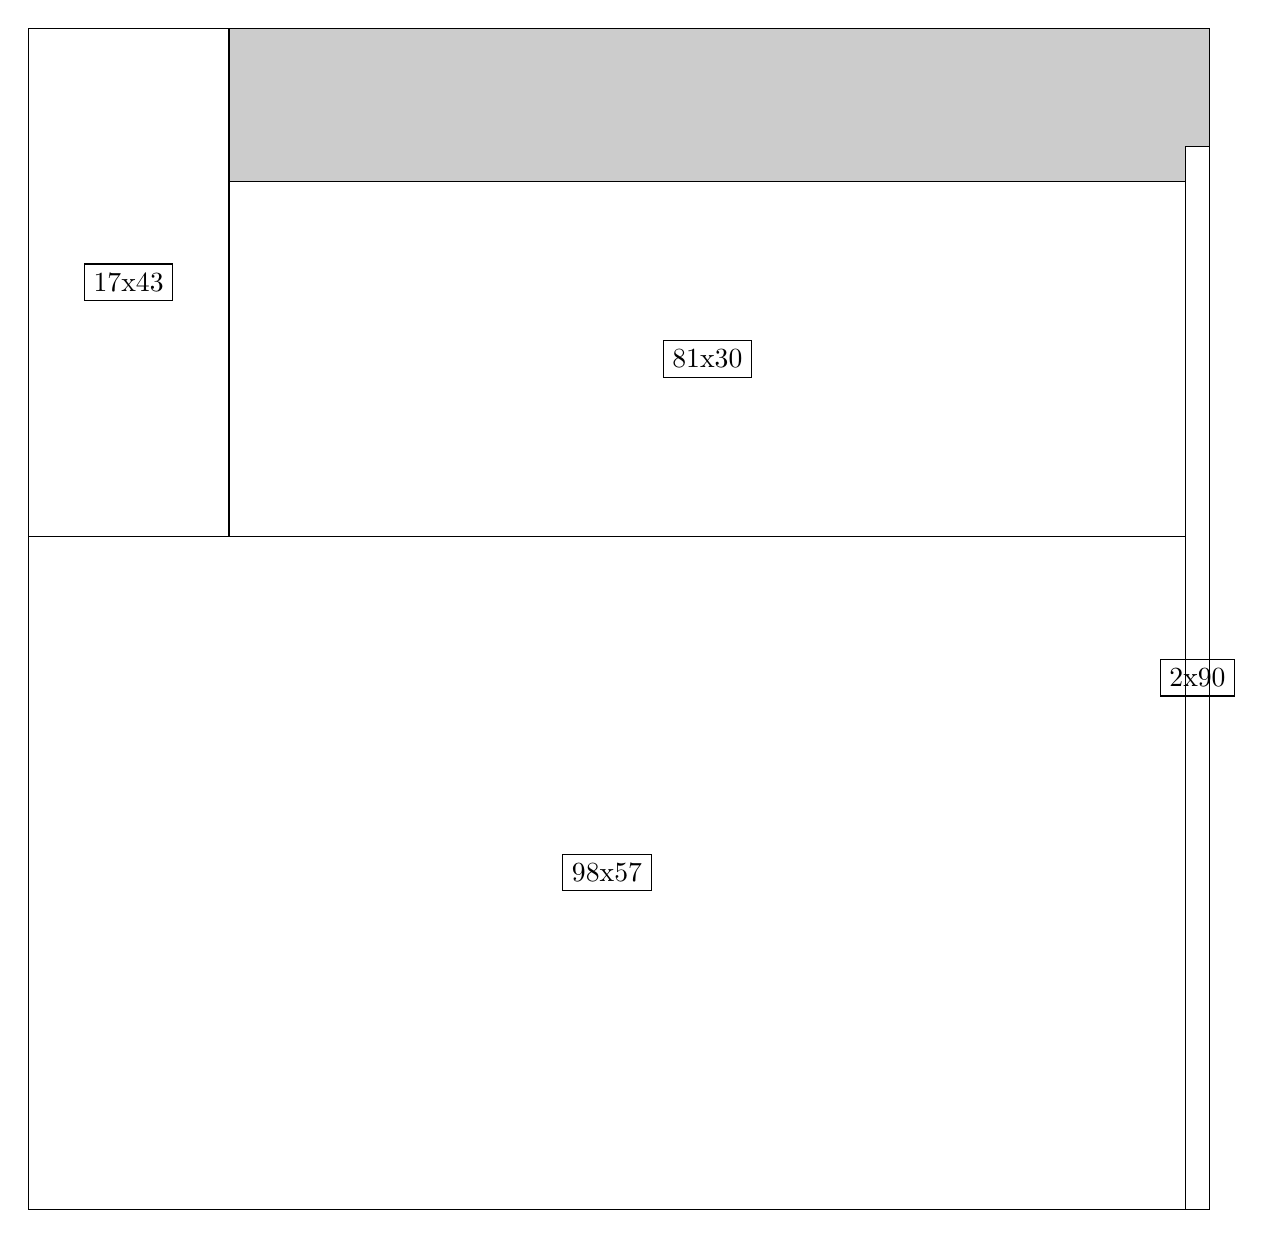
\begin{tikzpicture}[shorten >=1pt,scale=1.0,every node/.style={scale=1.0},->]
\tikzstyle{vertex}=[circle,fill=black!25,minimum size=14pt,inner sep=0pt]
\filldraw[fill=gray!40!white, draw=black] (0,0) rectangle (15.0,15.0);
\foreach \name/\x/\y/\w/\h in {98x57/0.0/0.0/14.7/8.549999999999999,81x30/2.55/8.549999999999999/12.15/4.5,2x90/14.7/0.0/0.3/13.5,17x43/0.0/8.549999999999999/2.55/6.45}
\filldraw[fill=white!40!white, draw=black] (\x,\y) rectangle node[draw] (\name) {\name} ++(\w,\h);
\end{tikzpicture}


w =98 , h =57 , x =0 , y =0 , v =5586
\par
w =81 , h =30 , x =17 , y =57 , v =2430
\par
w =2 , h =90 , x =98 , y =0 , v =180
\par
w =17 , h =43 , x =0 , y =57 , v =731
\par
\newpage


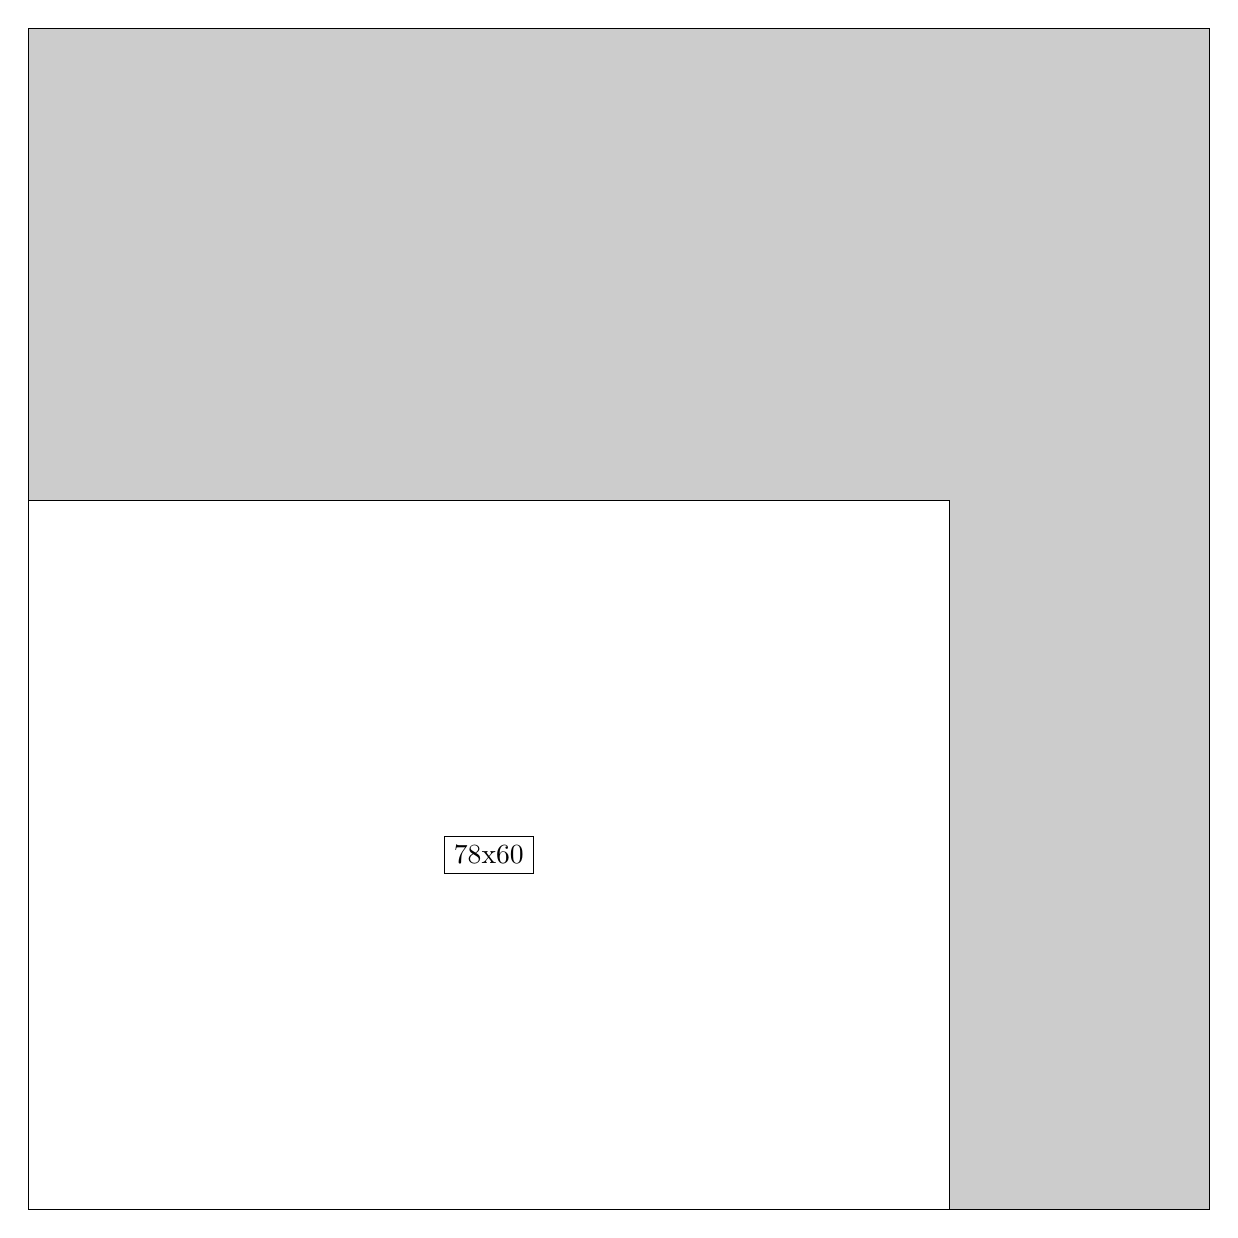
\begin{tikzpicture}[shorten >=1pt,scale=1.0,every node/.style={scale=1.0},->]
\tikzstyle{vertex}=[circle,fill=black!25,minimum size=14pt,inner sep=0pt]
\filldraw[fill=gray!40!white, draw=black] (0,0) rectangle (15.0,15.0);
\foreach \name/\x/\y/\w/\h in {78x60/0.0/0.0/11.7/9.0}
\filldraw[fill=white!40!white, draw=black] (\x,\y) rectangle node[draw] (\name) {\name} ++(\w,\h);
\end{tikzpicture}


w =78 , h =60 , x =0 , y =0 , v =4680
\par
\newpage


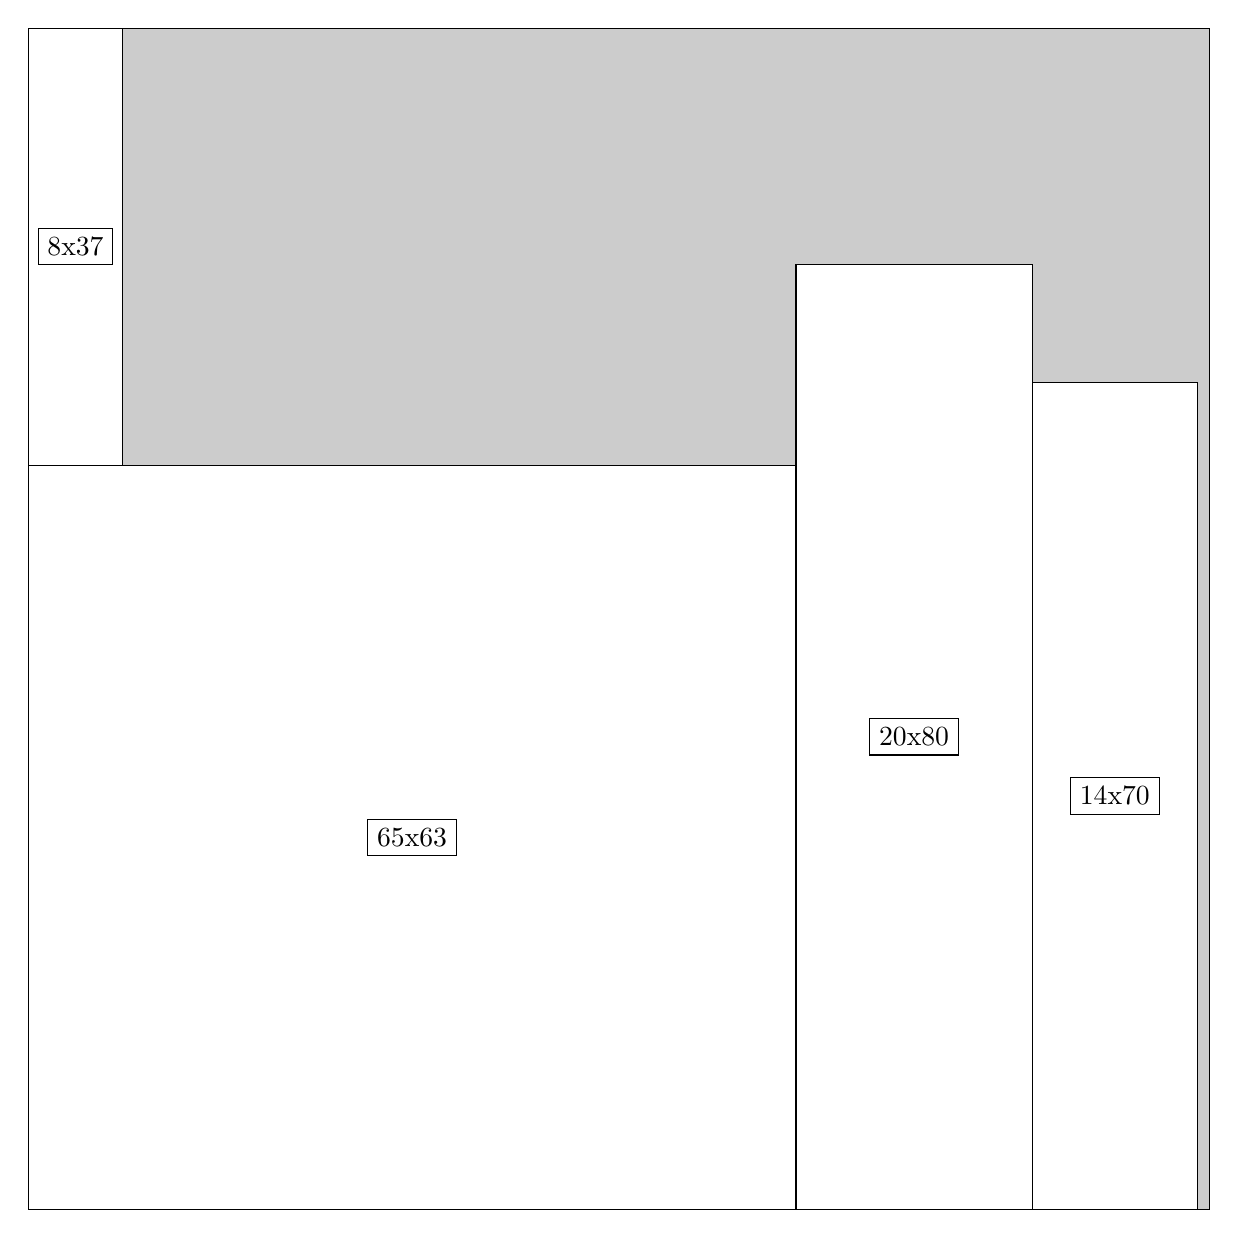
\begin{tikzpicture}[shorten >=1pt,scale=1.0,every node/.style={scale=1.0},->]
\tikzstyle{vertex}=[circle,fill=black!25,minimum size=14pt,inner sep=0pt]
\filldraw[fill=gray!40!white, draw=black] (0,0) rectangle (15.0,15.0);
\foreach \name/\x/\y/\w/\h in {65x63/0.0/0.0/9.75/9.45,20x80/9.75/0.0/3.0/12.0,14x70/12.75/0.0/2.1/10.5,8x37/0.0/9.45/1.2/5.55}
\filldraw[fill=white!40!white, draw=black] (\x,\y) rectangle node[draw] (\name) {\name} ++(\w,\h);
\end{tikzpicture}


w =65 , h =63 , x =0 , y =0 , v =4095
\par
w =20 , h =80 , x =65 , y =0 , v =1600
\par
w =14 , h =70 , x =85 , y =0 , v =980
\par
w =8 , h =37 , x =0 , y =63 , v =296
\par
\newpage


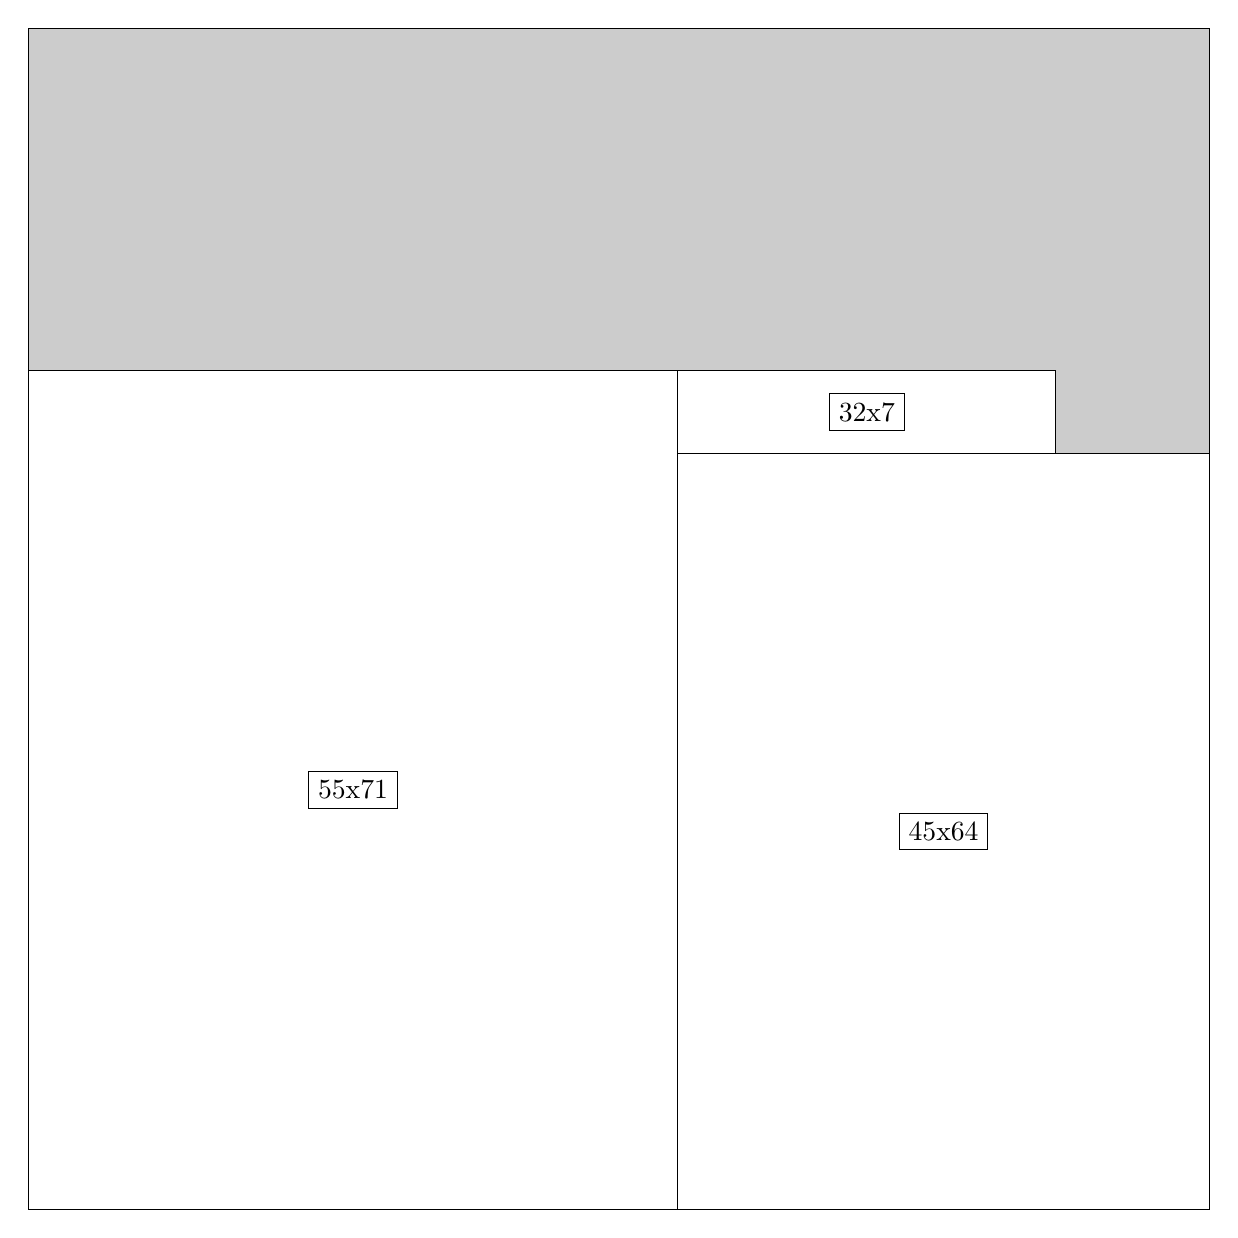
\begin{tikzpicture}[shorten >=1pt,scale=1.0,every node/.style={scale=1.0},->]
\tikzstyle{vertex}=[circle,fill=black!25,minimum size=14pt,inner sep=0pt]
\filldraw[fill=gray!40!white, draw=black] (0,0) rectangle (15.0,15.0);
\foreach \name/\x/\y/\w/\h in {55x71/0.0/0.0/8.25/10.65,45x64/8.25/0.0/6.75/9.6,32x7/8.25/9.6/4.8/1.05}
\filldraw[fill=white!40!white, draw=black] (\x,\y) rectangle node[draw] (\name) {\name} ++(\w,\h);
\end{tikzpicture}


w =55 , h =71 , x =0 , y =0 , v =3905
\par
w =45 , h =64 , x =55 , y =0 , v =2880
\par
w =32 , h =7 , x =55 , y =64 , v =224
\par
\newpage


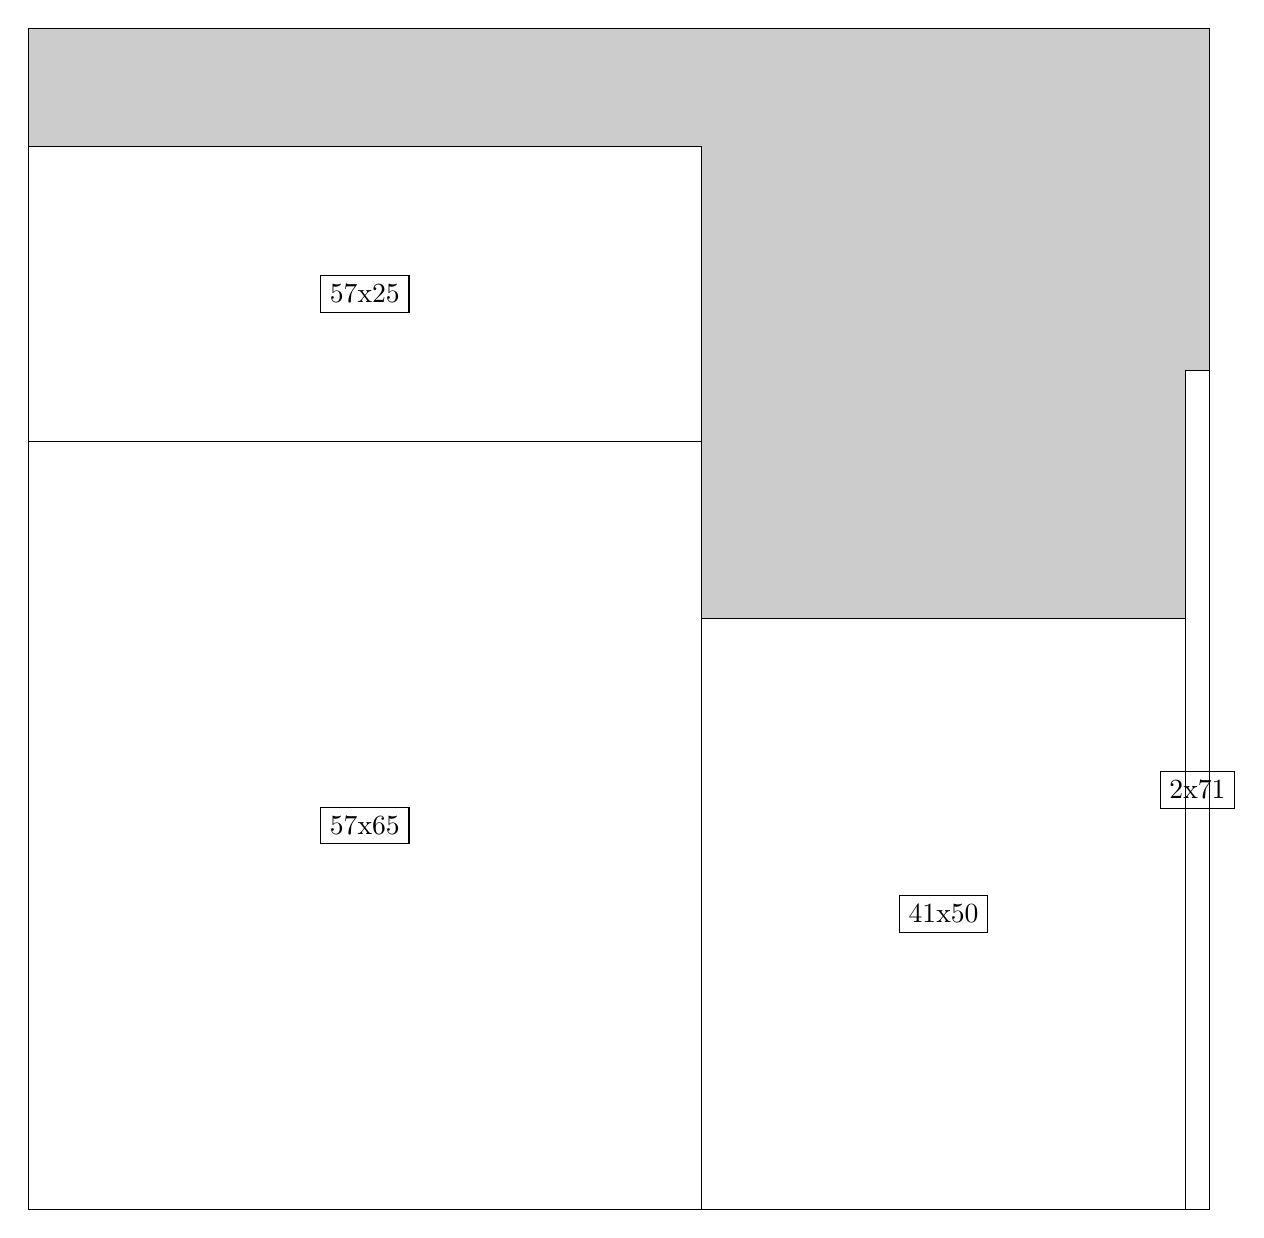
\begin{tikzpicture}[shorten >=1pt,scale=1.0,every node/.style={scale=1.0},->]
\tikzstyle{vertex}=[circle,fill=black!25,minimum size=14pt,inner sep=0pt]
\filldraw[fill=gray!40!white, draw=black] (0,0) rectangle (15.0,15.0);
\foreach \name/\x/\y/\w/\h in {57x65/0.0/0.0/8.549999999999999/9.75,41x50/8.549999999999999/0.0/6.1499999999999995/7.5,57x25/0.0/9.75/8.549999999999999/3.75,2x71/14.7/0.0/0.3/10.65}
\filldraw[fill=white!40!white, draw=black] (\x,\y) rectangle node[draw] (\name) {\name} ++(\w,\h);
\end{tikzpicture}


w =57 , h =65 , x =0 , y =0 , v =3705
\par
w =41 , h =50 , x =57 , y =0 , v =2050
\par
w =57 , h =25 , x =0 , y =65 , v =1425
\par
w =2 , h =71 , x =98 , y =0 , v =142
\par
\newpage


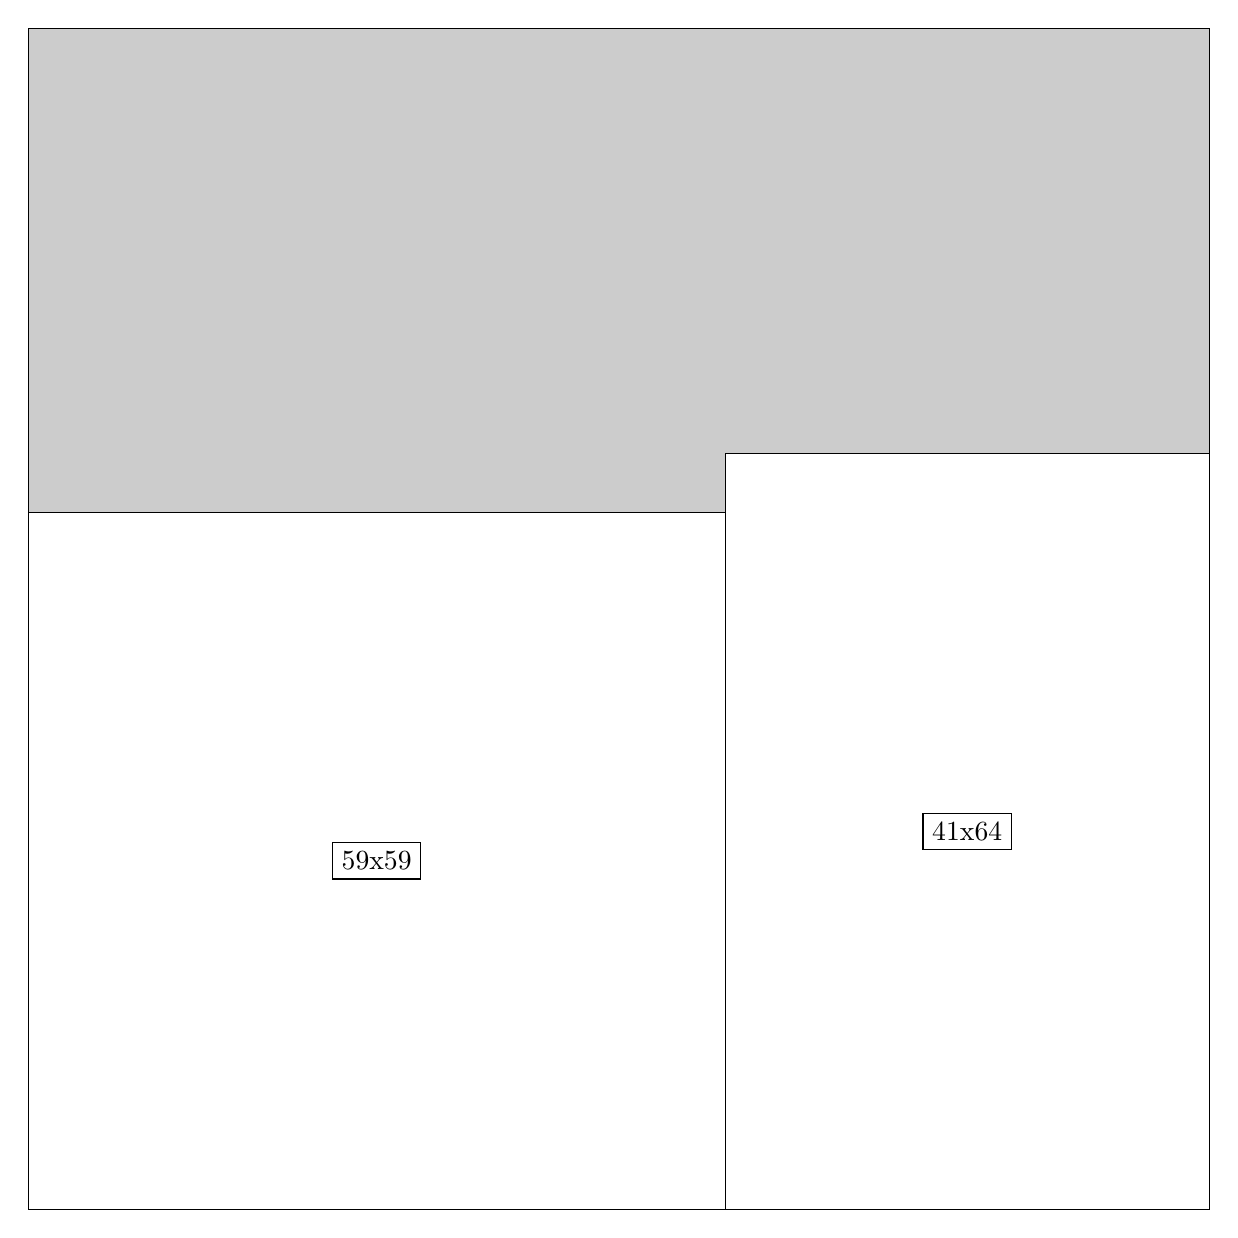
\begin{tikzpicture}[shorten >=1pt,scale=1.0,every node/.style={scale=1.0},->]
\tikzstyle{vertex}=[circle,fill=black!25,minimum size=14pt,inner sep=0pt]
\filldraw[fill=gray!40!white, draw=black] (0,0) rectangle (15.0,15.0);
\foreach \name/\x/\y/\w/\h in {59x59/0.0/0.0/8.85/8.85,41x64/8.85/0.0/6.1499999999999995/9.6}
\filldraw[fill=white!40!white, draw=black] (\x,\y) rectangle node[draw] (\name) {\name} ++(\w,\h);
\end{tikzpicture}


w =59 , h =59 , x =0 , y =0 , v =3481
\par
w =41 , h =64 , x =59 , y =0 , v =2624
\par
\newpage


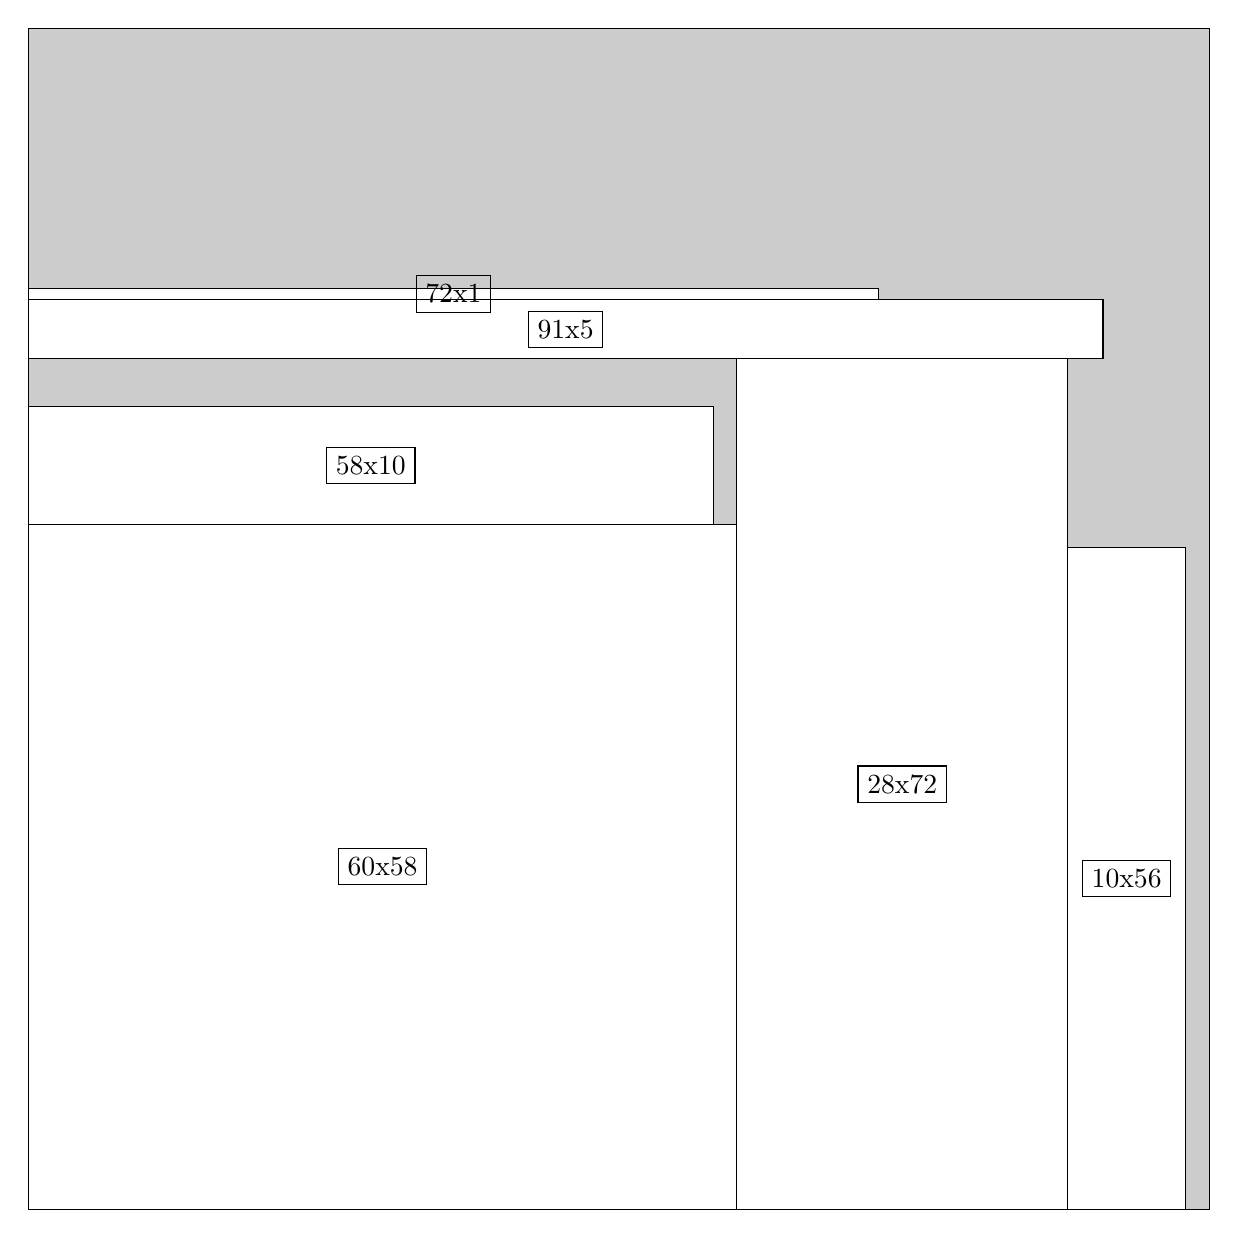
\begin{tikzpicture}[shorten >=1pt,scale=1.0,every node/.style={scale=1.0},->]
\tikzstyle{vertex}=[circle,fill=black!25,minimum size=14pt,inner sep=0pt]
\filldraw[fill=gray!40!white, draw=black] (0,0) rectangle (15.0,15.0);
\foreach \name/\x/\y/\w/\h in {60x58/0.0/0.0/9.0/8.7,28x72/9.0/0.0/4.2/10.799999999999999,58x10/0.0/8.7/8.7/1.5,10x56/13.2/0.0/1.5/8.4,91x5/0.0/10.799999999999999/13.65/0.75,72x1/0.0/11.549999999999999/10.799999999999999/0.15}
\filldraw[fill=white!40!white, draw=black] (\x,\y) rectangle node[draw] (\name) {\name} ++(\w,\h);
\end{tikzpicture}


w =60 , h =58 , x =0 , y =0 , v =3480
\par
w =28 , h =72 , x =60 , y =0 , v =2016
\par
w =58 , h =10 , x =0 , y =58 , v =580
\par
w =10 , h =56 , x =88 , y =0 , v =560
\par
w =91 , h =5 , x =0 , y =72 , v =455
\par
w =72 , h =1 , x =0 , y =77 , v =72
\par
\newpage


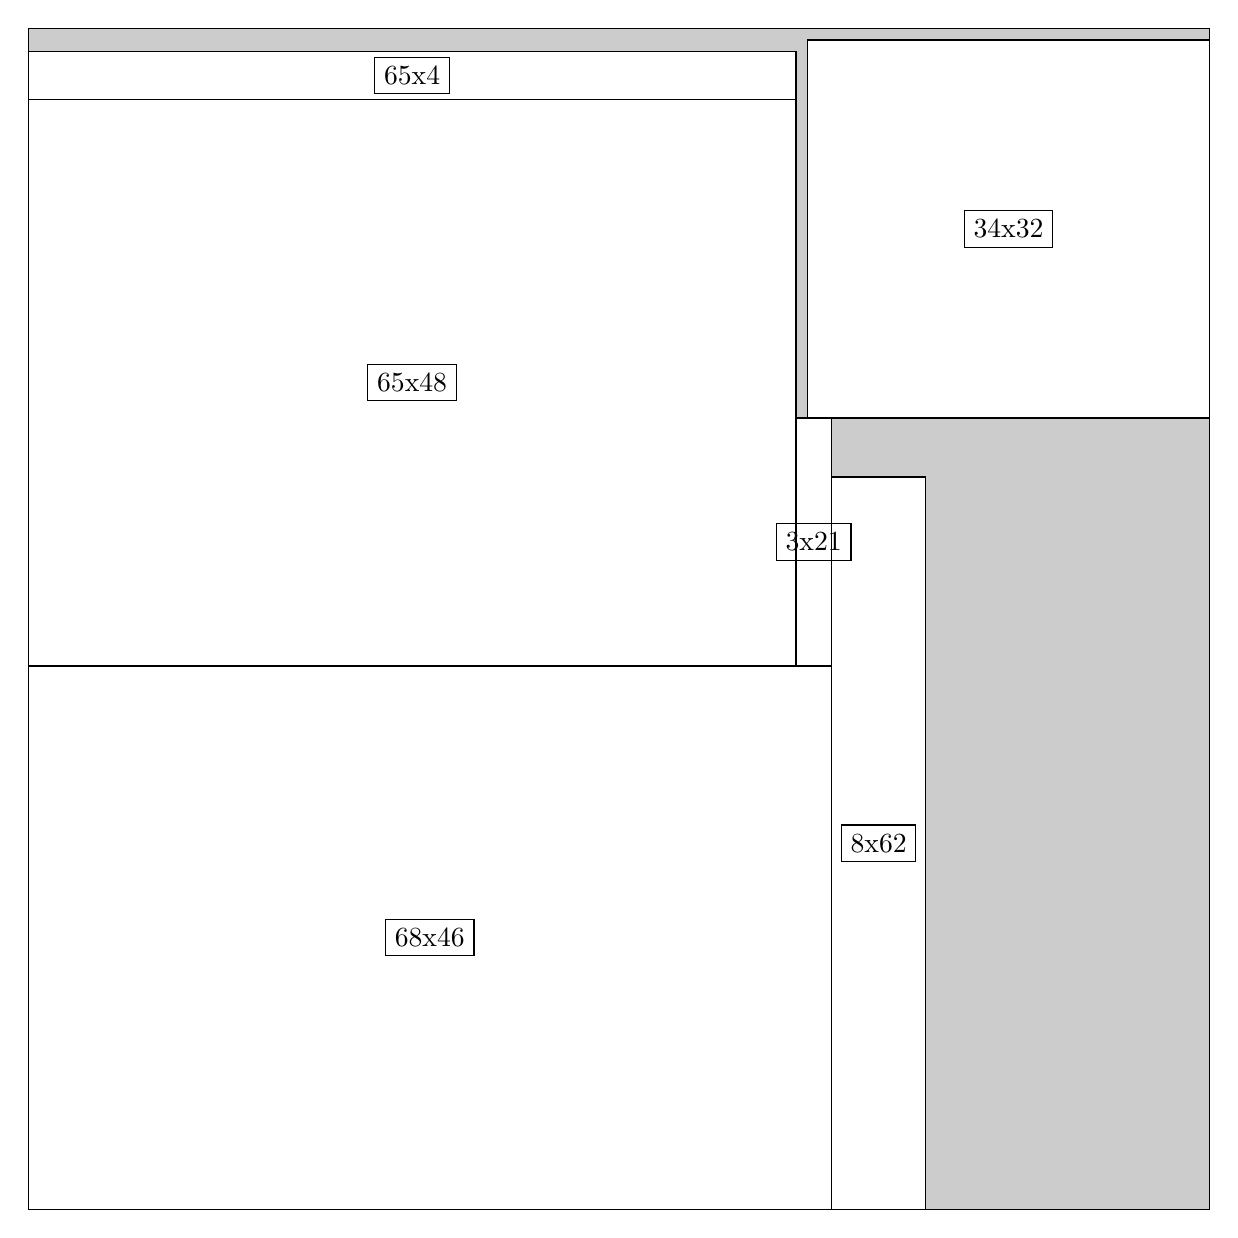
\begin{tikzpicture}[shorten >=1pt,scale=1.0,every node/.style={scale=1.0},->]
\tikzstyle{vertex}=[circle,fill=black!25,minimum size=14pt,inner sep=0pt]
\filldraw[fill=gray!40!white, draw=black] (0,0) rectangle (15.0,15.0);
\foreach \name/\x/\y/\w/\h in {68x46/0.0/0.0/10.2/6.8999999999999995,65x48/0.0/6.8999999999999995/9.75/7.199999999999999,34x32/9.9/10.049999999999999/5.1/4.8,8x62/10.2/0.0/1.2/9.299999999999999,65x4/0.0/14.1/9.75/0.6,3x21/9.75/6.8999999999999995/0.44999999999999996/3.15}
\filldraw[fill=white!40!white, draw=black] (\x,\y) rectangle node[draw] (\name) {\name} ++(\w,\h);
\end{tikzpicture}


w =68 , h =46 , x =0 , y =0 , v =3128
\par
w =65 , h =48 , x =0 , y =46 , v =3120
\par
w =34 , h =32 , x =66 , y =67 , v =1088
\par
w =8 , h =62 , x =68 , y =0 , v =496
\par
w =65 , h =4 , x =0 , y =94 , v =260
\par
w =3 , h =21 , x =65 , y =46 , v =63
\par
\newpage


\end{document}